\chapter{基于双目立体视觉的NLOS IS-VLP系统}
\section{系统概述}
本章在前一章的基础上,通过对硬件系统进行改进,设计了一个基于双目立体视觉的NLOS IS-VLP系统,并且给出了系统流程、实验设计以及性能测试。首先,由于双目立体视觉算法可以实现在已知一个点在左右目图像上的像素坐标的情况下,可以计算其在相机坐标系的坐标。因此,本系统通过双目相机只需要捕获LED关于地面的对称点来进行VLP。在惯性测量单元(IMU)的辅助下又可以获得相机的姿态,通过计算机视觉算法很容易实现基于单灯的NLOS IS-VLP系统。

\section{双目立体视觉算法}
本方案利用双目相机实现单点定位,在只需要一个LED的情况下可以实现3D定位。本文将在这里给出基于双目立体视觉算法的定位原理。已知空间中一点在左目右目相机上的投影点的像素坐标,双目立体视觉算法可以用来计算空间中的这一点在左目或者右目相机坐标系CCS中的3D坐标。假设,空间中的一点$P$在左目和右目CCS中的坐标分别是$\mathbf{P_{l}}$ 和 $\mathbf{P_{r}}$,如图所示,它们之间的关系由下式给出:
\begin{equation}\label{Pl=RPr+T}
\mathbf{P_{l}=RP_{r}+T}
\end{equation}
其中, $\mathbf{R}$ 和 $\mathbf{T}$分别是右目相机相对于左目相机的旋转矩阵和平移向量,它们的值可以通过对双目相机标定得到。假设$P$点在左目和右目相机照片上的投影点为$P_{1}$ 和 $P_{2}$,它们的值为($u_{1}$, $v_{1}$)和 ($u_{2}$, $v_{2}$)。用${z_{l}}$ 和 ${z_{r}}$分别表示$\mathbf{P_{l}}$ 和 $\mathbf{P_{r}}$的Z轴坐标,像素坐标系PCS和CCS之间存在关系入下:
\begin{equation}\label{zlzruv}
\begin{cases} 
  z_{l}\mathbf{t_{1}=K_{l}P_{l}}  \\
  z_{r}\mathbf{t_{2}=K_{r}P_{r}}                      
\end{cases}
\end{equation}
其中,$\mathbf{t_{1}}$=($u_{1}$, $v_{1}$,1),$\mathbf{t_{2}}$=($u_{2}$, $v_{2}$,1);$\mathbf{K_{l}}$ 和 $\mathbf{K_{r}}$分别是左目和右目相机的内参矩阵。通过求解方程(\ref{Pl=RPr+T})和 (\ref{zlzruv}),可以计算出$\mathbf{P_{l}}$的值。
\begin{figure*}[!htbp]
  \centering
  \includegraphics[width=0.8\linewidth]{FIG/dualcamera.pdf}
 \caption{双目立体视觉模型}
\label{fig:dualcamera}
\end{figure*}
可以建立关于点$P$从世界坐标系WCS到左目CCS的转换关系:
\begin{equation}\label{PlPw}
\mathbf{P_{l}=R_{l}P_{w}+T_{l}}
\end{equation}
其中,$\mathbf{R_{l}}$ 和 $\mathbf{T_{l}}$分别是WCS相对于左目CCS的旋转矩阵和平移向量。由此,可以得到左目相机的焦点在WCS中的位置:
\begin{equation}\label{wl}
\mathbf{W_{l}=-R_{l}^{-1}T_{l}}
\end{equation}
注意,左目相机的焦点在WCS中的位置也就是本系统的目标位置。

在 方程(\ref{PlPw})和(\ref{wl})中$\mathbf{R_{l}}$的值可以通过一个惯性测量单元IMU测量得到,由此,通过方程(\ref{PlPw})可以计算出$\mathbf{T_{l}}$。然后再代入到方程(\ref{wl})中,目标位置即可求解。在多数情况下,由于相机参数误差、系统测量误差和PCS中投影坐标的估计误差,方程组(\ref{Pl=RPr+T})和 (\ref{zlzruv})可能没有实数解。因此,在这项工作中,本系统将解方程组 (\ref{Pl=RPr+T})和 (\ref{zlzruv})转换成找$P_{1}$ 和 $P_{2}$的重投影误差的最小值。对于2D重投影误差函数,存在一个求解最小值点的最优解,其给出为:
\begin{equation}\label{pl^*}
\mathbf{P_{l}}^\ast = \arg\min _{\mathbf{P_{l}}} \left \{ 
\begin{Vmatrix}
\mathbf{t_{1}-K_{l}P_{l}}/z_{l}
\end{Vmatrix}^{2}
+
\begin{Vmatrix}
\mathbf{t_{2}-K_{r}R^{-1}(P_{l}-T)}/z_{r}
\end{Vmatrix}^{2}
\right \} 
\end{equation}
最后,可以获得相应的目标位置表达式,如下所示:
\begin{equation}\label{wl*}
\mathbf{W_{l}^{*}=P_{w}-R_{l}^{-1}P_{l}^{*}}
\end{equation}

\section{误差补偿算法}
\begin{figure}[!t]
\begin{minipage}{0.49\linewidth}
  \centerline{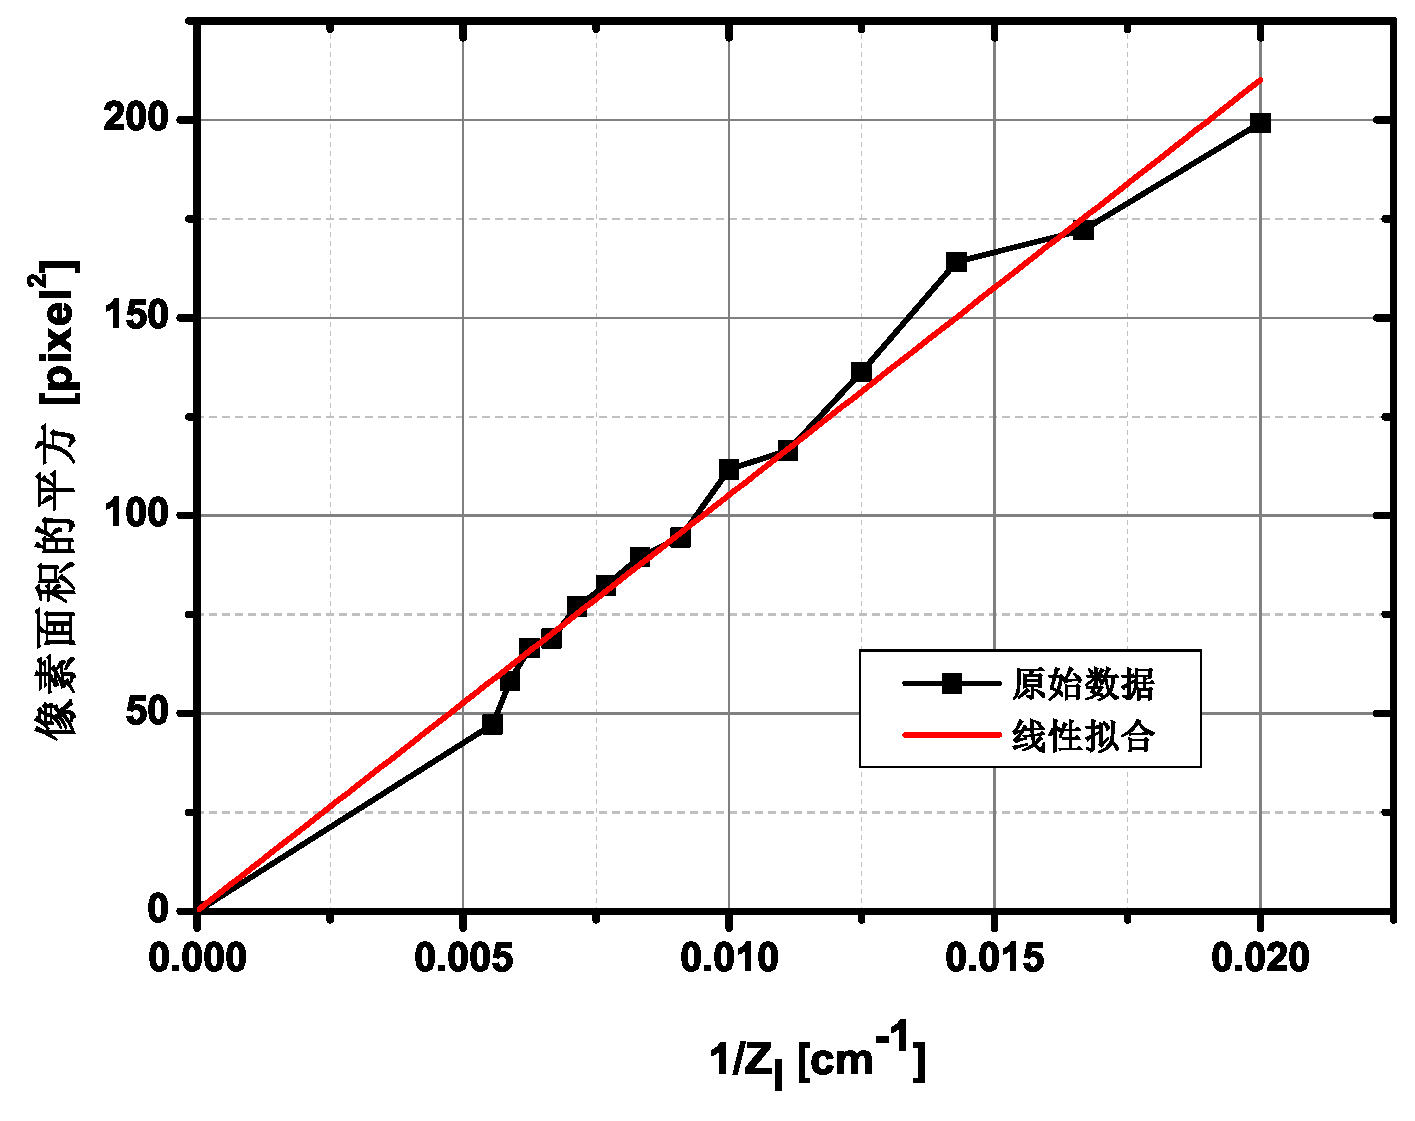
\includegraphics[width=\textwidth]{FIG/5-12b.eps}}
  \centerline{(a)}
\end{minipage}
\hfill
\begin{minipage}{0.49\linewidth}
  \centerline{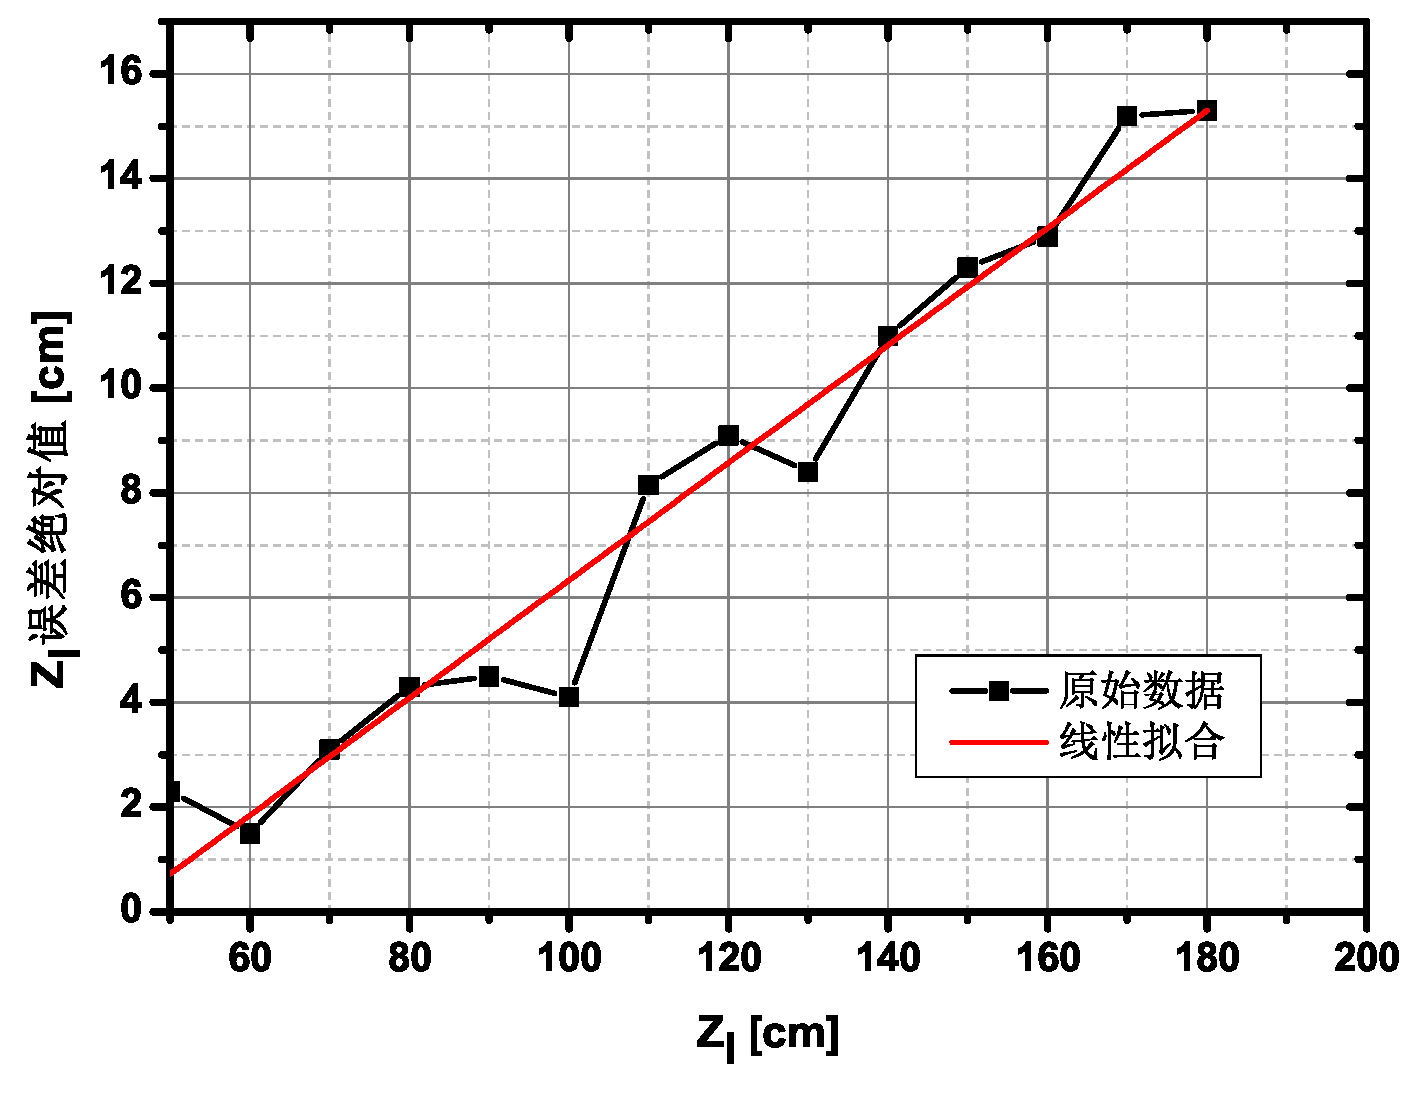
\includegraphics[width=\textwidth]{FIG/5-12a.eps}}
  \centerline{(b)}
\end{minipage}
\vfill
\caption{误差分析: (a)对称点附近高亮区域面积的平方和$z_{l}$倒数的线性拟合,(b)$z_{l}$误差绝对值与$z_{l}$}
\label{fig:erroranlysiszw}
\end{figure}
从公式(\ref{pl^*})和(\ref{wl*})可以看出,系统误差有三个主要来源,分别是相机参数、IMU角度估计和PCS上对称点的估计误差。为了简化误差分析,本系统暂不考虑来自相机参数和IMU角度估计的系统误差部分,只关注对称点的估计误差对系统性能的影响,并提出了一个误差补偿算法来补偿它。因此,本系统首先通过公式(\ref{pl^*})和(\ref{wl*})给出系统误差函数,如下所示:
\begin{equation}\label{delta wl*}
\Delta\mathbf{ W_{l}=W_{l}^{*}-W_{l}^{'}=R_{l}^{-1}(P_{l}^{'}-P_{l}^{*})=R_{l}^{-1}}\Delta \mathbf{P_{l}}
\end{equation}
其中$\Delta\mathbf{ W_{l}}$是系统误差,包括$x$、$y$和$z$轴上的估计误差,$\mathbf{W_{l}{'}}$是所提出的系统的估计值。$\mathbf{P_{l}{'}}$和$\Delta\mathbf{ P_{l}}$分别是点$P$在左相机CCS上的估计值和估计误差。由于忽略了IMU角度估计误差,等式(\ref{delta wl*})中的$\mathbf{R_{l}}$的值可以确定。大量研究工作表明,在$\Delta\mathbf{ P_{l}}$中, $z $ 轴上的估计误差比 $ x $ 和 $ y $ 轴上的大得多,这也与实验中的结果一致。因此,我们认为 $ z_ { l } $ 的估计误差是影响系统误差的最重要因素。因此,我们设计了一个针对双目视觉的NLOS IS-VLP系统的误差补偿(Error Compensation, EC)算法,通过优化 $ z_ { l } $ 来补偿 $ z $ 轴上的系统误差。在EC中,我们只讨论了 $ z_ { l } $ 的误差。将公式(\ref{Pl=RPr+T})和(\ref{zlzruv})展开成方程形式,可以将 $ z_ { l } $ 表示为:   
\begin{equation}\label{xlylzl}
  {z_{l}=f_{lx}f_{rx}t_{0}/(f_{rx}(u_{1}-u_{l})-f_{lx}(u_{2}-u_{r}))}	
\end{equation}
其中$u_{l}$是左相机焦点在PCS上的投影的横坐标,$f_{lx}$是左相机的焦距与每个像素长度的比值,$u_{r}$,$f_{rx}$类似。我们选择$z_{l}^{'}$作为$z_{l}$的测量值,$\Delta z_{l}$被视为$z_{l}$的误差,表示为:
\begin{equation}\label{xl'yl'zl'}
  \Delta z_{l}=z_{l}-z_{l}^{'}= z_{l}z_{l}^{'}(f_{lx}\Delta u_{2}-f_{rx}\Delta u_{1})/ f_{lx}f_{rx}t_{0}
\end{equation}
其中$\Delta u_{1}$和$\Delta u_{2}$分别是$u_{1}$和$u_{2}$的估计误差。显然,PCS上对称点周围高亮区域的像素面积大小会随着$z_{l}$的增加而减小。这一点在图\ref{fig:erroranlysiszw}(a)中得到了实验验证。注意,根据相对误差的一致性,可以认为$\Delta u_{1}$、$\Delta u_{2}$和$z_{l}$之间存在反比关系。通过这种关系,$\Delta z_{l}$在公式(\ref{xl'yl'zl'})下与$z_{l}^{'}$呈线性关系。
 
本系统建立了一个实验测试平台,其中LED固定在距离地面40 cm的高度,相机朝向LED的反射点,以确保$\mathbf{R_{l}}$是单位矩阵,消除了IMU角度估计误差的影响。图\ref{fig:erroranlysiszw}(b)显示了$\Delta z_{l}$与$z_{l}$之间的绝对值的测量数据点和线性拟合,它们是线性关系。注意,得到的结果受到相机灵敏度和地板平整度的影响。相机ISO设置为50,以确保可以捕捉和检测到LED边缘。考虑到线性效应不明显,$z$轴上的误差随着相机到LED对称点的距离的增加而增加。因此,为了补偿误差,使用线性拟合的系数$\lambda=0.112$,如下所示:
 \begin{equation}\label{ECzl}
 {z_{l}^{*}=z_{l}^{'}(1+\sigma \lambda/(1-\lambda ) ) }
\end{equation}
其中,$\sigma$的取值只能是“1”或者“0”,它被用来决定$z_{l}$的测量值是否需要被优化。

EC算法的实现流程如图\ref{fig:EC-BPE}所示,其中$H$是PCS上对称点周围的高亮区域。假设$\sigma=1$,可以通过公式(\ref{zlzruv})计算$(u_{1},v_{1})$和$(u_{2},v_{2})$,然后由公式(\ref{ECzl})计算$z_{l}=z_{l}^{*}$。注意,($i $)如果两者都在对称点周围的高亮区域内,则$\sigma=1$,否则$\sigma=0$;($ii $)确定了$\sigma$后,可以优化$z_{l}$;以及($iii $)然后,通过将其代入公式(\ref{wl})来确定EC算法下的目标值。
\begin{figure}[!t]
\centering\includegraphics[width=\textwidth]{FIG/EC procedure.pdf}
\caption{EC算法流程图}
\label{fig:EC-BPE}
\end{figure}





\section{系统方案}

所提出方案的系统模型如图\ref{fig:dualcam_systemscheme}所示,主要由NLOS OCC子系统和基于双目立体视觉的单点定位子系统组成,其中NLOS OCC系统的实验过程在第三章已经详述,通过它来实现对LED坐标的提取。对于位置估计子系统,本系统提出了两种不同的方案,都是在只有一个LED的情况下实现3D NLOS IS-VLP。第一种是将LED在地面上的对称点视为点$P$来估计相机位置。这种方案系统性能会随着地面粗糙度的增加而降低。当粗糙程度过大时,图像检测高光亮点可能失败。为了克服这个问题,本系统提出了一种地标增强(Label Enhanced, LBE)的可见光成像定位方案(LBE IS-VLP),将方案一中的点$P$替换为标签,该标签是LED在反射表面上的正投影,需要提前标记。与NLOS IS-VLP通过像素灰度值检测高亮区域相比,LBE IS-VLP通过标签的形状来识别标签,因此粗糙反射面对其影响较小。
\begin{figure*}[!t]
  \centering
  \includegraphics[width=0.85\linewidth]{FIG/systemscheme.pdf}
 \caption{基于双目相机的NLOS IS-VLP系统模型}
\label{fig:dualcam_systemscheme}
\end{figure*}

第一种方案,在发射端LED光信号进行调制;在接收端双目相机通过切换长短曝光来实现通信和捕捉反射面的高光点。在通过NLOS OCC子系统获取到LED的坐标之后,很容易得到LED关于地面对称点的坐标即(${x_{0}}$,${y_{0}}$,$-z_{0}$),由于LED通过NLOS链路在左右摄像机上的投影等于对称点通过LOS链路的投影。将此对称点的坐标和其在左右目相机上的投影点坐标代入到双目立体视觉算法中,就可以计算出目标位置。通过边缘检测和椭圆拟合,可以得到此坐标。如图\ref{fig:dual_imageprocessing}(a)所示,可以将拟合椭圆的中心点坐标作为对称点在左右目相机上的投影点坐标。
\begin{figure*}[!htbp]
\begin{minipage}{0.75\linewidth}
  \centerline{\includegraphics[width=\textwidth]{FIG/imageprocessing.pdf}}
  \centerline{(a)}
  \label{fig:imageprocessing-a}
\end{minipage}
\hfill
\begin{minipage}{0.23\linewidth}
  \centerline{\includegraphics[width=\textwidth]{FIG/cornerdetecting.pdf}}
  \centerline{(b)}
  \label{fig:imageprocessing-b}
\end{minipage}
\vfill
\caption{参考点坐标提取: (a) 椭圆拟合提取高光点坐标;(b) 角点检测标签位置}
\label{fig:dual_imageprocessing}
\end{figure*}


LBE IS-VLP方案基本上与NLOS IS-VLP相同,只是将双目视觉算法中的点$P$替换为标签,该标签是LED在反射面上的正投影,在实验之前进行标记。因此,在LBE IS-VLP中,可以根据LED坐标计算标签在世界坐标系上的坐标。与NLOS IS-VLP一样,也可以使用NLOS OCC子系统接收LED坐标。同时,可以使用双目相机来识别标签。这种方案涉及的详细过程与NLOS IS-VLP非常相似,只是将标签视为参考点。标签的世界坐标系下的坐标由标签和LED之间的几何关系确定,即(${x_{0}}$, ${y_{0}}$,${0}$)。本方案使用了角点检测方法来处理来自左右相机的照片,从而检测标签,标签在像素坐标系上的坐标是四个角点坐标的平均值,见图\ref{fig:dual_imageprocessing}(b)。
 
\section{实验与性能}
\subsection{实验环境}
所提出的系统的实验测试平台如图\ref{fig:dual_environment-setup}所示。发射端由工作频率为3.3 kHz的STM32微控制器单元、驱动模块和LED组成,LED位于距地面1.96 m的高度,其在地面上投影点是WCS的原点。在接收端,使用ZED2双目相机捕捉左右相机的两幅图像,而IMU用于测量相机姿态。首先,本系统校准了ZED2以获得其两个相机的内部参数矩阵。经过内参标定,发现两个相机之间的旋转矩阵基本上近似是一个单位矩阵,相机之间只在x轴有位移。
\begin{figure}[!htbp]
\centering\includegraphics[width=0.7\textwidth]{FIG/experimentsetup.pdf}
\caption{实验硬件系统}
\label{fig:dual_environment-setup}
\end{figure}


因此,在(\ref{Pl=RPr+T})中有$\mathbf{R=I}$和$\mathbf{T}=[t_{0},0,0]$,其中$t_{0}$是一个常数。注意,对于每个实验,本系统都调整了ZED2的位置,以确保它在地板上的投影的位置与一个测试点重合。本系统测量了ZED的高度作为测试点z轴坐标。通过比较测试点的坐标和使用所提出的系统估计的ZED2的坐标,确定了系统误差。本系统对总共60个点进行了这样的操作并估计了RMSE和误差CDF。所有使用的关键系统参数都给出在表\ref{tab:dual_parameter}中。
\begin{table}[!htbp]
	\centering  
	\caption{基于双目视觉的NLOS VLP系统实验参数}  
	\label{tab:dual_parameter}   
	\begin{tabular}{lc}  
        \toprule
        \makebox[0.35\linewidth][l]{$\textbf{实验参数}$} &\makebox[0.5\linewidth][c]{$\textbf{参数值}$}\\ 
        \midrule
		测试环境& 200 $\times$ 200 $\times$ 196 $\mathrm{cm^{3}}$ \\
		MCU 输出频率& 3.3 kHz \\
		LED 输出功率&1.4 W\\
		LED 工作电压&5 V\\
		LED 坐标&(0,0,196) \\ 
		Label 坐标&(0,0,0) \\ 
		IMU 自由度&9 \\
		双目相机尺寸&3840 $\times$ 1080 \\
		双目相机相对位置&(12,0,0)  \\
		\bottomrule
	\end{tabular}
\end{table}

\subsection{系统性能}
通过所提出的系统的估计值和测量值之间的差的绝对值,确定了60个数据集的3D平均定位误差和RMSE。实验结果如表\ref{tab:systemerror}所示,其中最低的3D平均误差和RMSE分别为37.2和44.6 cm。此外,我们还计算了60个数据集的X、Y和Z轴上的平均误差,分别为6.96、6.01和35.32 cm。
  \begin{table}[!htbp]
                \centering  
                \caption{各种方案的性能比较}  
	\label{tab:systemerror}   
                \begin{tabular}{lccccc}  
                  \toprule 
                \makebox[0.15\linewidth][l]{$\textbf{方案}$} &\makebox[0.1\linewidth][c]{$\textbf{X (cm)}$}&\makebox[0.1\linewidth][c]{$\textbf{Y (cm)}$}&\makebox[0.1\linewidth][c]{$\textbf{Z (cm)}$}&\makebox[0.15\linewidth][c]{$\textbf{平均误差 (cm)}$}&\makebox[0.15\linewidth][c]{$\textbf{RMSE (cm)}$}\\ 
                \midrule  
                  NLOS IS-VLP &6.96&6.01&35.32&37.27&44.59 \\
		EC NLOS IS-VLP&6.96&6.01&22.58&26.10&31.02 \\ 
		LBE IS-VLP &3.62&3.24&4.50&7.31&7.74 \\
                  \bottomrule 
                \end{tabular}
\end{table}


图\ref{fig:2Derrorcompensation}描绘了NLOS IS-VLP在X-Y平面上的2D定位性能,从中可以看出,NLOS IS-VLP系统对于X-Y平面上的性能总体较好,除了一些远离LED的测试点有较大的偏差。图\ref{fig:NLOS VLP system error}显示了X、Y和Z轴以及3D的CDF图。 X 和 Y 轴上的CDF与图\ref{fig:2Derrorcompensation}的结果基本上一致,可以实现在90$\%$的置信度下小于 15 cm的定位精度。


\begin{figure}[!htbp]
\centering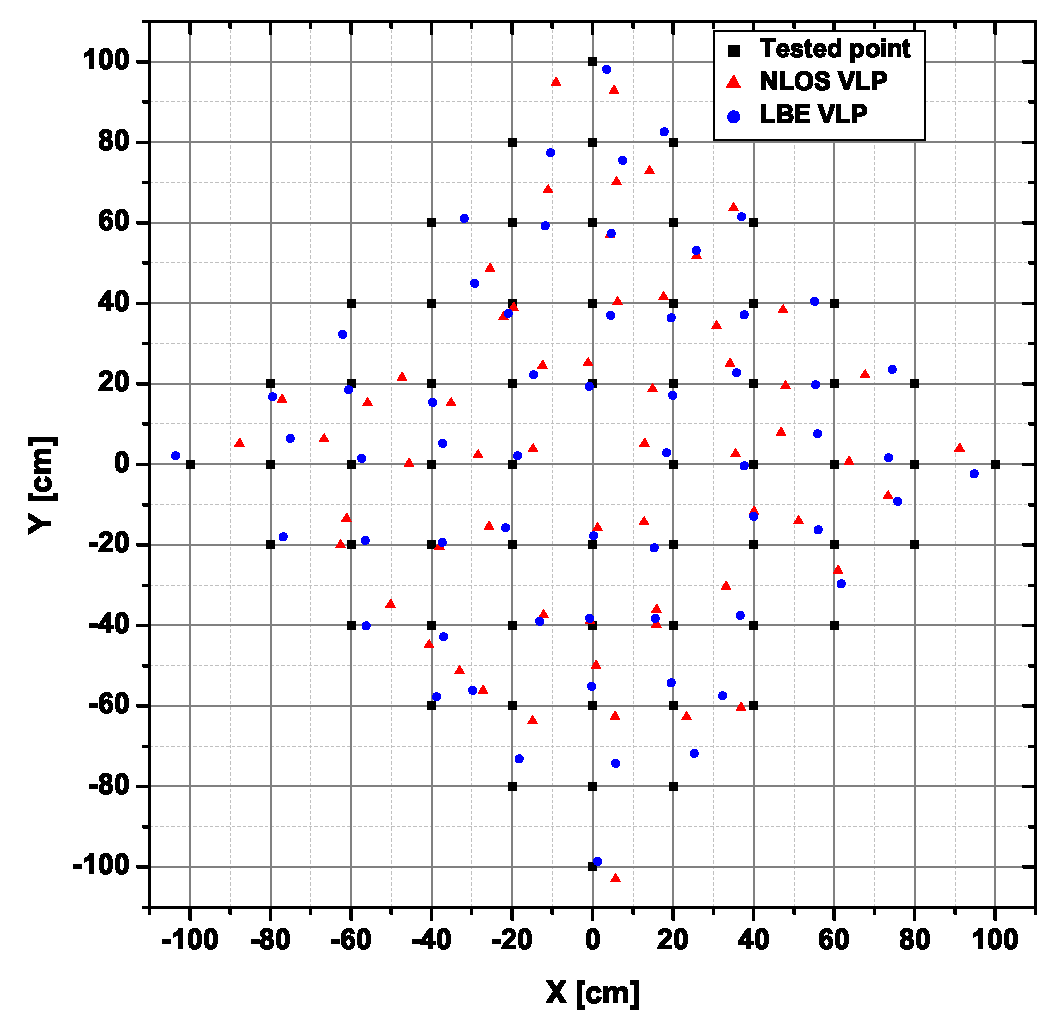
\includegraphics[width=0.65\textwidth]{FIG/2derror2.eps}
\caption{各种方案2D误差对比}
\label{fig:2Derrorcompensation}
\end{figure}

\begin{figure}[!htbp]
\centering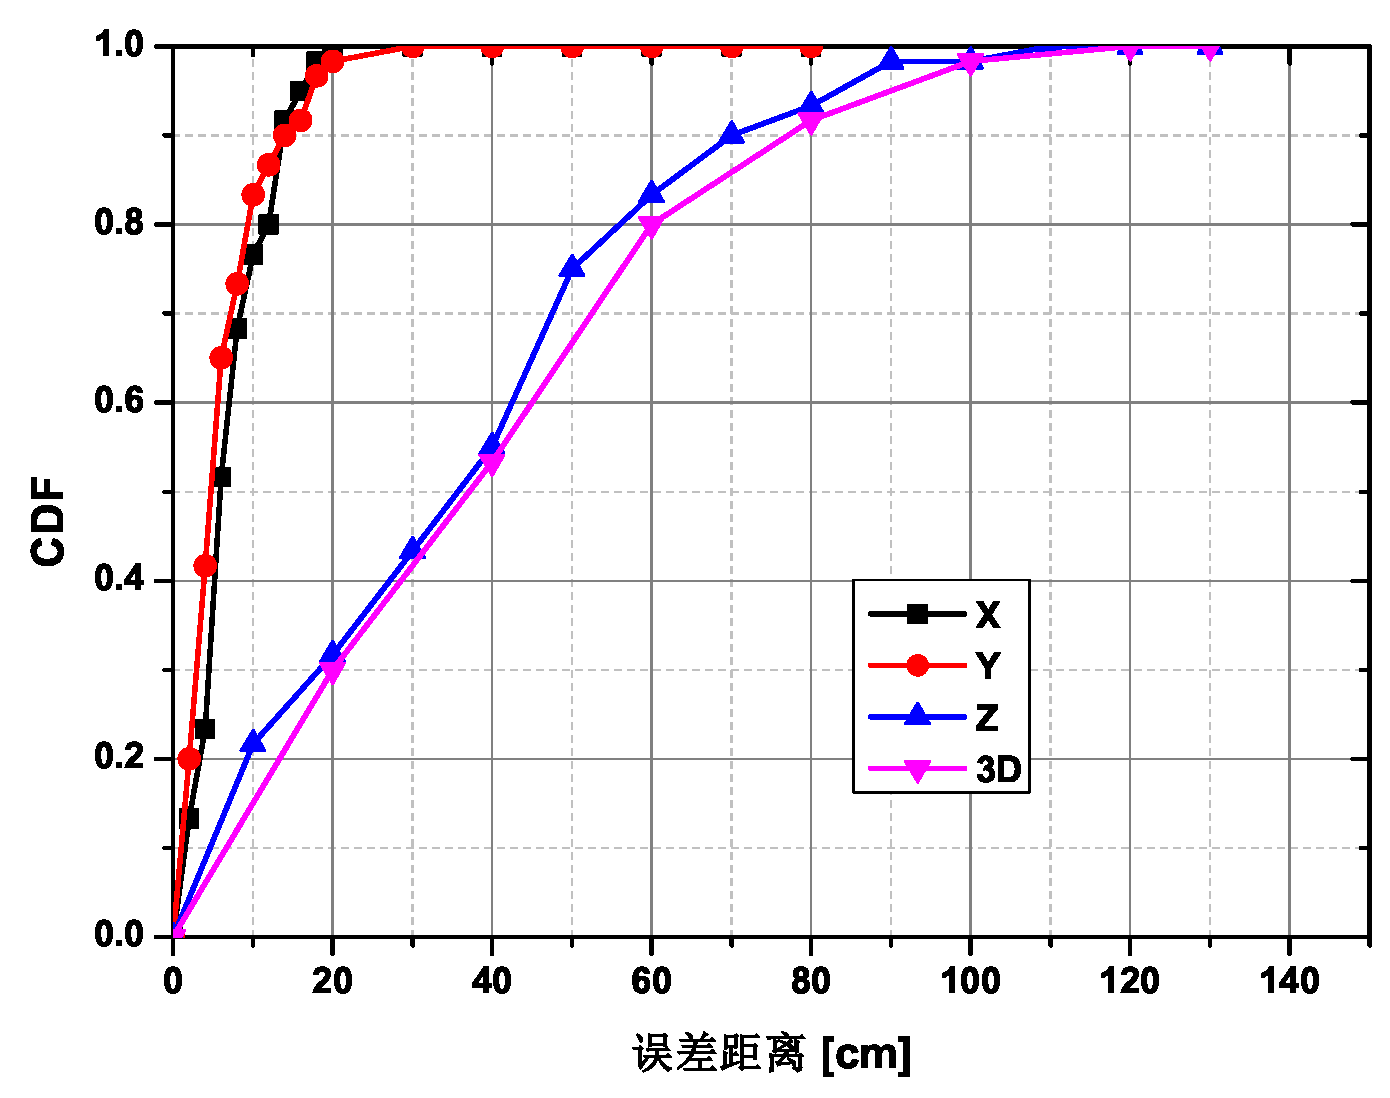
\includegraphics[width=0.65\textwidth]{FIG/517-b.eps}
\caption{NLOS IS-VLP系统X、Y和Z轴以及3D的CDF}
\label{fig:NLOS VLP system error}
\end{figure}


然而,对于 Z 轴和 3D的 CDF来说,在80$\%$的置信度下小于60 cm的定位精度并不令人满意。与没有经过误差补偿的NLOS IS-VLP相比,经过误差补偿的NLOS IS-VLP系统的最低平均误差和 RMSE 值分别降低至 26.10 和 31.02 cm。注意,在90$\%$的置信度下3D定位误差已经降到50 cm, 此外, CDF 曲线显示了误差补偿算法的效果,见图 \ref{fig:errorcompensation}。
\begin{figure}[!t]
\centering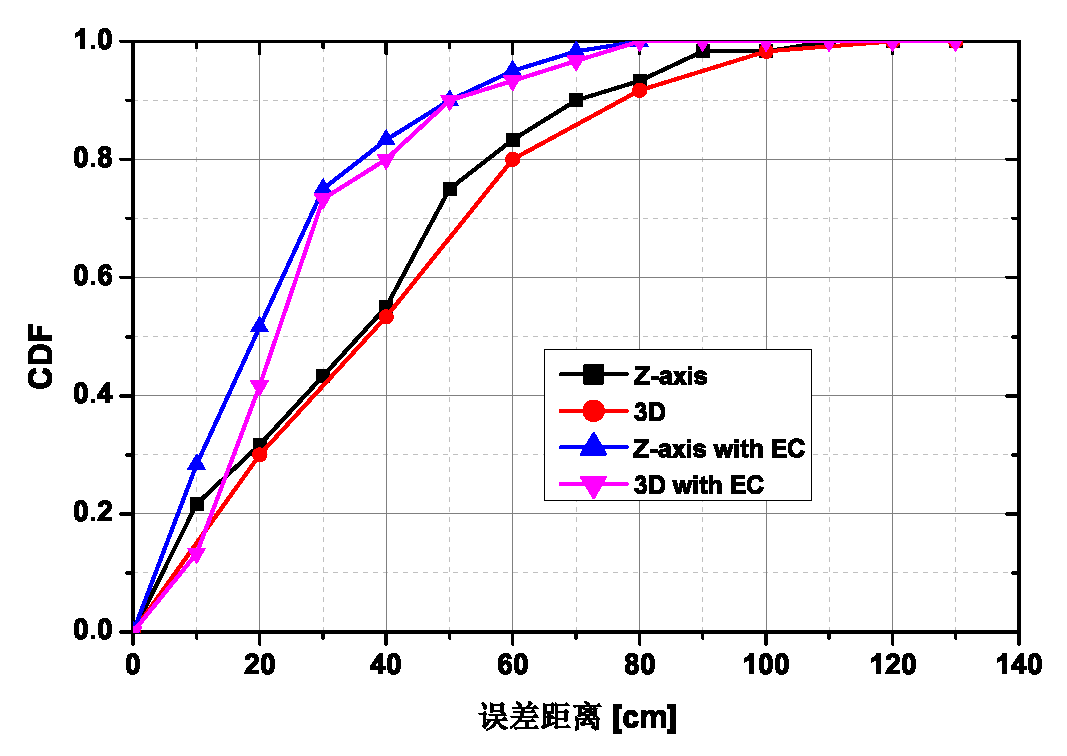
\includegraphics[width=0.65\textwidth]{FIG/518.eps}
\caption{有无误差补偿的CDF对比}
\label{fig:errorcompensation}
\end{figure}

\begin{figure}[!t]
\centering\includegraphics[width=0.65\textwidth]{FIG/519.eps}
\caption{LBE VLP方案:X、Y和Z轴以及3D的CDF}
\label{fig:cdflabel}
\end{figure}


同样的,系统对LBE IS-VLP方案进行了测试、测量和性能评估,与NLOS IS-VLP相同,估计了60组数据的RMSE和平均定位误差。实验结果如表\ref{tab:systemerror}所示,其中最低平均误差和RMSE分别为7.31和7.74 cm;X、Y和Z轴上的平均误差分别为3.62、3.24和4.50 cm。图\ref{fig:cdflabel}显示了X、Y和Z轴以及3D的CDF图,其中X、Y和Z轴都可以实现在90$\%$的置信度下小于8 cm的精度,而3D的性能可以实现在90$\%$的置信度下小于11 cm的精度。



\begin{figure}[!t]
\centering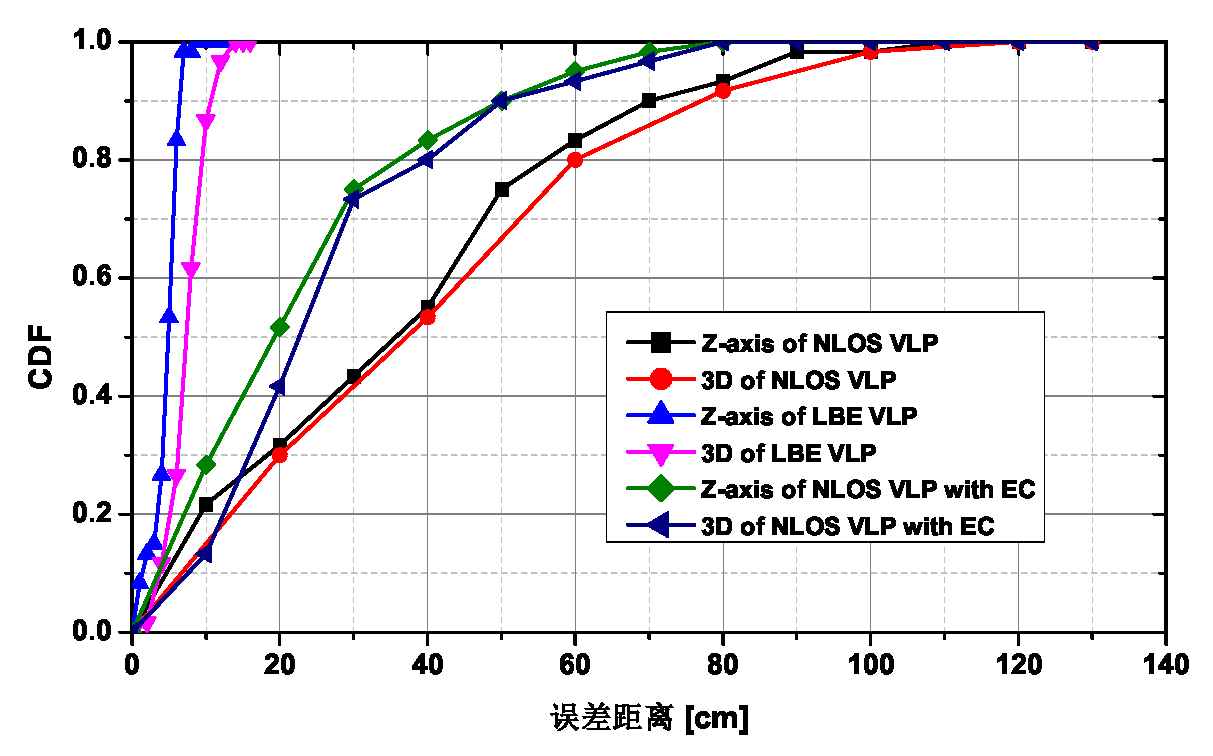
\includegraphics[width=0.65\textwidth]{FIG/520b.eps}
\caption{几种方案Z轴以及3D的CDF比较}
\label{fig:comparation}
\end{figure}


与NLOS IS-VLP相比,LBE IS-VLP在X-Y平面上距离LED较远的测试点明显提高了性能,见图\ref{fig:2Derrorcompensation}。图\ref{fig:comparation}描绘了LBE IS-VLP、NLOS IS-VLP和带有EC算法的NLOS IS-VLP几种方案下X、Y和Z轴以及3D的CDF性能。LBE IS-VLP具有参考点(标签或对称点)在像素坐标系上的估计误差较小,以及在相机坐标系上的估计误差较小,因为对称点到相机的距离比标签到相机的距离大得多。因此,从图\ref{fig:comparation}可以明显看出,与NLOS IS-VLP相比,LBE IS-VLP方案具有最佳性能。
 
 与LOS VLP相比,所提出的系统克服了LOS链路阴影或遮挡以及LED数量的限制,在仅有一个LED的情况下可以实现较高精度的定位。与所提出的基于亮度分布模型的NLOS VLP系统相比,通过改进接收端可以提高NLOS VLP系统的性能。



\section{本章小结}
 本章所提出的基于双目立体视觉的NLOS IS-VLP系统是在前一章的基础上,通过对硬件系统以及实验方案进行改进,来提高系统性能的。首先,本章介绍了基于双目立体视觉的定位算法,通过对误差进行分析给出了一个误差补偿算法。在此之后,给出了两种试验方案,以及实验测试了它们各自的性能。虽然,本文所提出的NLOS IS-VLP可以实现任意姿态的3D定位,但是定位性能依旧有待提高,虽然通过误差补偿,系统性能有所提高,但是,跟LBE IS-VLP方案相比,性能差距明显。然而,LBE IS-VLP方案需要提前进行标签的标注。总的来说,本系统成功的克服了本文开篇提出的VLP系统面临的两个主要难点,并且得到了一个较为可观的性能。